\documentclass[12pt]{article}

\usepackage{pablo}
\usepackage{pgfplots}
\usepackage{numprint}
\usepackage[a4paper,margin=2cm]{geometry}
\usetikzlibrary{calc}

\pagestyle{empty}
\begin{document}

\begin{center}
  {\large
    Devoir surveillé --- 1h

    \textsc{Statistiques --- Vecteurs}
  }

  Nom : \hfill ~
\end{center}

\begin{exercice}[Vecteurs --- 8 points]
  $ABC$ est un triangle quelconque. Les points $D$, $E$, $F$, $G$, $H$ sont définis par :
  $\vecteur{AD}= \dfrac{5}{4}\vecteur{AB}$ ;
  $\vecteur{AE}= \dfrac{1}{4}\vecteur{AB}$ ;
  $\vecteur{AF}=-\dfrac{3}{4}\vecteur{AB}$ ;
  $\vecteur{AG}= \dfrac{1}{2}\vecteur{BA}$ ;
  $\vecteur{AH}= 2\vecteur{BC} - \dfrac{1}{2}\vecteur{AC}$.

  \begin{center}
    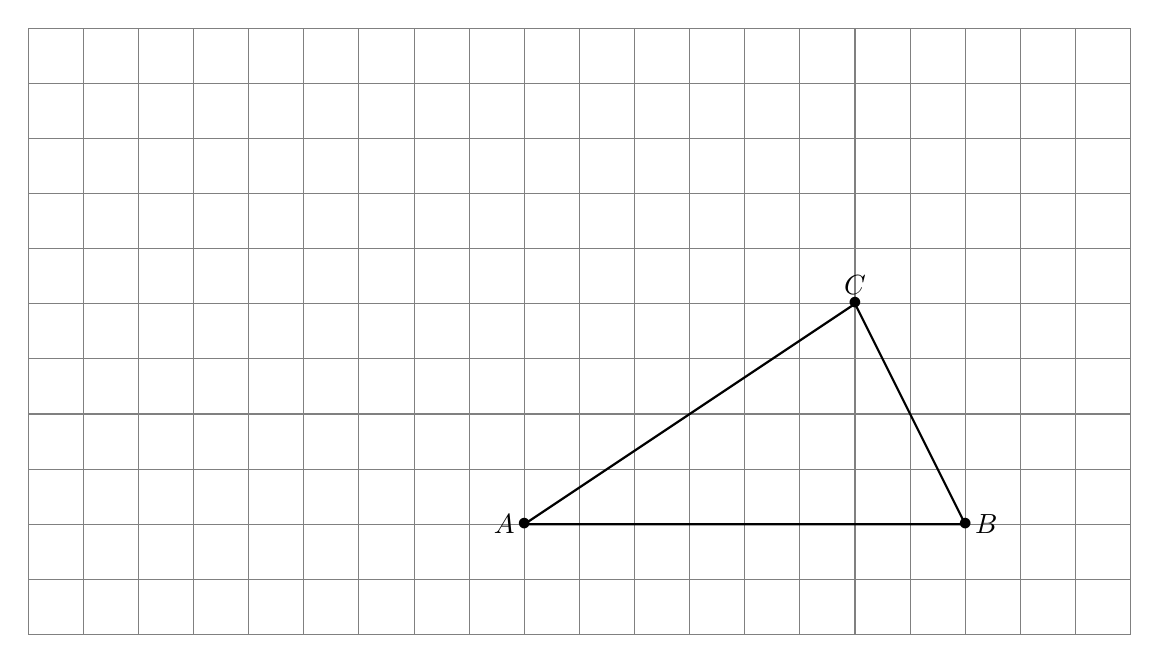
\begin{tikzpicture}[scale=0.7]
      \draw[thin,color=gray,step=1] (0,0) grid (20,11);
      \coordinate (A) at (9,2);
      \coordinate (B) at (17,2);
      \coordinate (C) at (15,6);
      \draw[thick] (A) -- (B) -- (C) -- cycle;
      \draw (A) node{$\bullet$} node[left]{$A$};
      \draw (B) node{$\bullet$} node[right]{$B$};
      \draw (C) node{$\bullet$} node[above]{$C$};

      %\coordinate (D) at ($5/4*(B)-1/4*(A)$);
      %\draw (D) node[below]{$D$} node{$\bullet$};

      %\coordinate (E) at ($1/4*(B)+3/4*(A)$);
      %\draw (E) node[below]{$E$} node{$\bullet$};

      %\coordinate (F) at ($-3/4*(B)+7/4*(A)$);
      %\draw (F) node[below]{$F$} node{$\bullet$};

      %\coordinate (G) at ($3/2*(A)-1/2*(B)$);
      %\draw (G) node[below]{$G$} node{$\bullet$};

      %\coordinate (H) at ($(A)+2*(C)-2*(B)-1/2*(C)+1/2*(A)$);
      %\draw (H) node[above]{$H$} node{$\bullet$};

    \end{tikzpicture}
  \end{center}

  \begin{enumerate}[(1)]
      \item Construire les points $D$, $E$, $F$, $G$ et $H$ sur la figure ci-dessus.
      \item
      \begin{enumerate}[(a)]
        \item Montrer, à l'aide de la relation de Chasles, que $\vecteur{ED}=\vecteur{AB}$.
        \item Montrer, à l'aide de la relation de Chasles, que $\vecteur{EF}=-\vecteur{AB}$.
        \item Que peut-on en déduire pour le point $E$ ? Justifier.
      \end{enumerate}
      \item
      \begin{enumerate}[(a)]
        \item Montrer, à l'aide de la relation de Chasles, que $\vecteur{GH}=\dfrac{1}{2}\vecteur{AB}+2\vecteur{BC}-\frac{1}{2}\vecteur{AC}$.
        \item En déduire une expression de $\vecteur{GH}$ en fonction du vecteur $\vecteur{BC}$.
        \item Que peut-on en déduire pour les vecteurs $\vecteur{GH}$ et $\vecteur{BC}$ ?
        \item Que peut-on en déduire pour les droites $(GH)$ et $(BC)$ ?
      \end{enumerate}
  \end{enumerate}
\end{exercice}

\begin{exercice}[Statistiques : Définitions ; Effectifs et fréquences --- 4 points]
  Claude Got (chercheur en accidentologie) a étudié les accidents de la route
  mortels, en fonction du type d'usager.

  En 1960, sur les \numprint{8295} tués, \numprint{2540} étaient automobilistes, et \numprint{848} étaient
  cyclistes. Presque cinquante ans plus tard, en 2007, sur les \numprint{4620} tués, \numprint{2464}
    étaient automobilistes, et \numprint{142} étaient cyclistes.

  \begin{enumerate}[(1)]
    \item Quelle est la population étudiée ? Quel est le caractère ? Est-il quantitatif ou qualitatif ?
    \item Quel était le pourcentage de cyclistes tués en 1960, en fonction du nombre total de tués ?
    \item Même question pour 2007.
  \end{enumerate}
\end{exercice}

\begin{exercice}[Statistiques : Lecture graphique ; Médiane --- 8 points]
  Voici la répartition des espérances de vie à la naissance de tous les pays
  du monde (source : \emph{CIA World Factbook}, 2013).

  \begin{center}
    \begin{tikzpicture}
      \begin{axis}[
          xscale=1.5,
          yscale=2,
          xmin=40,
          xmax=90,
          ymin=0,
          ymax=110,
          xlabel=Espérance de vie (années),
          y label style={below left},
          ylabel=Effectif (nombre de pays),
          grid=both,
          ybar interval,
          xminorgrids=false,
          xmajorgrids=false,
          ytick={0,10,...,110},
          minor ytick={0,5,...,110},
          extra y ticks={0,10,...,110},
          every extra y tick/.style={
            yticklabel pos=right,
          },
          minor grid style={gray},
          major grid style={black},
          xtick={40,50,...,90},% reset from ybar interval
          xticklabel={$[\pgfmathprintnumber\tick, \pgfmathprintnumber\nexttick[$}]],
        % a data file containing 8000 normally distributed
        % random numbers of mean 0 and variance 1
        \addplot+[hist={data=x,bins=5}] file {ds4-esperance.txt};
      \end{axis}
    \end{tikzpicture}
  \end{center}

  \begin{enumerate}[(1)]
    \item Combien de pays ont une espérance de vie à la naissance comprise entre 60 et 70 ans ?
    \item\label{moyenne} Quelle est la moyenne des espérance de vie de tous les pays du monde
      ? Pour le calcul, on considèrera les milieux des classes : par exemple,
      pour la classe $[70,80[$, on considèrera que les 100 pays de cette classe
          on une espérance de vie de 75 ans.
    \item
      \begin{enumerate}[(a)]
        \item Dresser le tableau des effectifs cumulés croissants.
        \item Quelle est la classe médiane ?
      \end{enumerate}
    \item
      \begin{enumerate}[(a)]
      \item L'espérance de vie à la naissance en France est 82 ans. La France fait-elle partie de la moitié des pays qui ont l'espérance de vie la plus haute ?
      \item L'espérance de vie en Russie est 70 ans. Quel pourcentage des pays du monde ont une espérance de vie plus élevée ?
    \end{enumerate}
  \item Peut-on affirmer que l'espérance de vie mondiale est égale à la valeur de la moyenne trouvée en question \ref{moyenne} ? Pourquoi ?
  \end{enumerate}

\end{exercice}


\begin{exercice}[Bonus --- 2 points]
  Cent élèves participent à une épreuve notée sur 20 ; la moyenne de toutes les notes est 10.
  Les garçons sont 50\% de plus que les filles, et la moyenne des filles est 50\% de plus que celle des garçons.
  \begin{enumerate}[(1)]
    \item Quel est le nombre de garçons et de filles ?
    \item Quel est la moyenne des filles et celle des garçons ?
  \end{enumerate}
\end{exercice}

\end{document}
